
\documentclass[12pt]{report}

\usepackage{fullpage}
\usepackage{graphicx}
\usepackage{listings}
\usepackage{verbatim}
\usepackage{amsmath}
\usepackage{color}
\usepackage{hyperref}
 
\definecolor{codegreen}{rgb}{0,0.6,0}
\definecolor{codegray}{rgb}{0.5,0.5,0.5}
\definecolor{codepurple}{rgb}{0.58,0,0.82}
\definecolor{backcolour}{rgb}{0.95,0.95,0.92}
 
\lstdefinestyle{mystyle}{
    backgroundcolor=\color{backcolour},   
    commentstyle=\color{codegreen},
    keywordstyle=\color{magenta},
    numberstyle=\tiny\color{codegray},
    stringstyle=\color{codepurple},
    basicstyle=\footnotesize,
    breakatwhitespace=false,         
    breaklines=true,                 
    captionpos=b,                    
    keepspaces=true,                 
    numbers=left,                    
    numbersep=5pt,                  
    showspaces=false,                
    showstringspaces=false,
    showtabs=false,                  
    tabsize=2
}

\lstdefinestyle{DOS}
{
    backgroundcolor=\color{black},
    basicstyle=\scriptsize\color{white}\ttfamily
}
 
\lstset{style=mystyle}
\renewcommand{\baselinestretch}{2}
\author{Mohammed Nauman Sididque}
\title{Assignment 4 \\Information Retrieval \\ CS 834 \\ Fall 2017 }

\begin{document}
\maketitle
\tableofcontents
\chapter{Problem 8.3}
\section{Problem Statement}
For one query in the CACM collection (provided at the book website), generate a ranking using Galago, and then calculate average precision, NDCG at 5 and 10, precision at 10, and the reciprocal rank by hand.
\section{Solution}
This problem uses CACM corpus provided in the test collection of the book. The queries ran against the CACM collection have been used from the processed queries section of the CACM test collection.\\

\subsection{Query:Interested in articles on robotics motion planning particularly the geometric and combinatorial aspects we are not interested in the dynamics of arm motion}

The below xml file shows the query which was used in galago for batch-search.\\
\lstinputlisting{Problem8_3/onequery.xml}

The below commands were run on command prompt for generating the ranked list of query with 10 results. 
\begin{lstlisting}[style=DOS]
F:\Fall2017\InformationRetreival\Assignment3\Galgo\galagosearch-1.04-bin\galagosearch-1.04\bin>galago.bat batch-search --index=F:\Fall2017\InformationRetreival\Assignment4\index.idx --count=10 F:\Fall2017\InformationRetreival\Assignment4\onequery.xml > F:\Fall2017\InformationRetreival\Assignment4\cacm_onequery.list
\end{lstlisting}

The below list file was generated by batch search from galago.
\verbatiminput{Problem8_3/cacm_onequery.list}

The below commands were run on galago to evaluate the ranked list for query generated from the previous step.
\begin{lstlisting}[style=DOS]
F:\Fall2017\InformationRetreival\Assignment3\Galgo\galagosearch-1.04-bin\galagosearch-1.04\bin> galago.bat eval F:\Fall2017\InformationRetreival\Assignment4\cacm_onequery.list  F:\Fall2017\InformationRetreival\Assignment4\cacm.rel >F:\Fall2017\InformationRetreiva\Assignment4\onequeryoutput.txt
\end{lstlisting}

The below text file is the result of eval command by using the relevance judgments file provided in cacm test collections.
\verbatiminput{Problem8_3/onequeryoutput.txt}

The calculation of precision for the ranking was done with the help of relevance judgements provided with the test collections. It contains list of all the documents relevant to a collection. Below is the list of relevant documents for query 6.

\verbatiminput{Problem8_3/relevancefeedback.rel}

\subsubsection{ Precision at 10}

$Precision(1) = 0/1 = 0$\\
$Precision(2) = 0/2 = 0$\\ 
$Precision(3) = 1/3 = 0.33$\\
$Precision(4) = 1/4 = 0.25$\\
$Precision(5) = 2/5 = 0.4$\\
$Precision(6) = 3/6 = 0.5$\\
$Precision(7) = 3/7 = 0.429$\\
$Precision(8) = 3/8 = 0.375$\\
$Precision(9) = 3/9 = 0.33$\\
$Precision(10) = 3/10 = 0.3$\\
where Precision(6) denotes precision at search result 6.\\
The Precision(10) for this query is 0.3. \\  

\subsubsection{Mean Average Precision}

$MAP = 1/3 (1/3 + 2/5 + 3/6) $\\
$MAP = 0.41$
\subsubsection{Reciprocal Rank}
The first relevant document is at position 3.\\
$RR = 1/3 $\\
$RR = 0.333$\\

\subsubsection{Normalized Discounted Cummulative Gain at 5}

Relevance Score: 0, 0, 1, 0, 1\\
$CG_5 = 0+ 0+ 1+ 0+ 1$\\
$CG_5 = 2$ \\
\begin{table}[]
\centering
\caption{Discounted Cummulative Gain}
\label{my-label}
\begin{tabular}{llll}
i & $rel_i$ & $log_2(i + 1)$   & $rel_i / log_2(i + 1)$  \\
1 & 0        & 1     		    & 0   \\
2 & 0        & 1.585 		    & 0 \\
3 & 1        & 2     		    & 0.5  \\
4 & 0        & 2.322 		    & 0 \\
5 & 1        & 2.585 		    & 0.387   
\end{tabular}
\end{table}
$DCG = \sum\limits_{i=1}^5 rel_i / log_2(i + 1)$ \\
$DCG = 0 + 0 + 0.5 + 0 + 0.387 =  0.887$\\

Ideal Discounted Cummulative Gain has the document and relevance score as below:\\
Relevance Score: 1, 1, 0, 0, 0\\
$CG_5 = 1+ 1+ 0+ 0+ 0$\\
$CG_5 = 2$ \\
\begin{table}[]
\centering
\caption{Ideal Discounted Cummulative Gain}
\label{my-label}
\begin{tabular}{llll}
i & $rel_i$ & $log_2(i + 1)$   & $rel_i / log_2(i + 1)$  \\
1 & 1        & 1     		    & 1    \\
2 & 1        & 1.585 		    & 0.631 \\
3 & 0        & 2     		    & 0  \\
4 & 0        & 2.322 		    & 0 \\
5 & 0        & 2.585 		    & 0   
\end{tabular}
\end{table}
$IDCG = \sum\limits_{i=1}^5 rel_i / log_2(i + 1)$ \\
$IDCG = 1 + 0.631 + 0 + 0 + 0 =  1.631$\\
Normalized Discounted Cummulative Gain (NDCG)=  DCG / IDCG\\
$NDCG = 0.887 / 1.631 = 0.544$

\subsubsection{Normalized Discounted Cummulative Gain at 10}

Relevance Score: 0, 0, 1, 0, 1, 1, 0, 0, 0, 0\\
$CG_{10} = 0+ 0+ 1+ 0+ 1 + 1 + 0 + 0 + 0 + 0$\\
$CG_{10}= 3$ \\
\begin{table}[]
\centering
\caption{Discounted Cummulative Gain}
\label{my-label}
\begin{tabular}{llll}
i & $rel_i$ & $log_2(i + 1)$   & $rel_i / log_2(i + 1)$  \\
1 & 0        & 1     		    & 0    \\
2 & 0        & 1.585 		    & 0 \\
3 & 1        & 2     		    & 0.5  \\
4 & 0        & 2.322 		    & 0 \\
5 & 1        & 2.585 		    & 0.387 \\ 
6 & 1        & 2.807     	    & 0.356    \\
7 & 0        & 3 		    & 1 \\
8 & 0        & 3.17    		    & 0  \\
9 & 0        & 3.22 		    & 0 \\
10 & 0      & 3.459 		    & 0 \\ 
\end{tabular}
\end{table}
$DCG = \sum\limits_{i=1}^{10} rel_i / log_2(i + 1)$ \\
$DCG = 0 + 0 + 0.5 + 0 + 0.387 + 0.356 + 0 + 0 + 0 + 0 =  1.243$\\
Ideal Discounted Cummulative Gain has the document and relevance score as below:\\
Relevance Score: 1, 1, 1, 0, 0, 0, 0, 0 , 0 , 0 \\
$CG_{10} = 1+ 1 + 1+ 0+ 0+ 0+ 0 + 0 + 0 + 0$\\
$CG_{10} = 3$ \\
\begin{table}[]
\centering
\caption{Ideal Discounted Cummulative Gain}
\label{my-label}
\begin{tabular}{llll}
i & $rel_i$ & $log_2(i + 1)$   & $rel_i / log_2(i + 1)$  \\
1 & 1        & 1     		    & 1    \\
2 & 1        & 1.585 		    & 0.61 \\
3 & 1        & 2     		    & 0.5  \\
4 & 0        & 2.322 		    & 0 \\
5 & 0        & 2.585 		    & 0 \\ 
6 & 0        & 2.807     	    & 0   \\
7 & 0        & 3 		    & 0 \\
8 & 0        & 3.17    		    & 0  \\
9 & 0        & 3.22 		    & 0 \\
10 & 0      & 3.459 		    & 0 \\ 
\end{tabular}
\end{table}
$IDCG = \sum\limits_{i=1}^{10} rel_i / log_2(i + 1)$ \\
$IDCG = 1 + 0.61 + 1 + 0.5 + 0 + 0 + 0 + 0 + 0 + 0 =  2.11$\\
Normalized Discounted Cummulative Gain (NDCG)=  DCG / IDCG\\
$NDCG = 1.243 / 2.11 = 0.589$

\chapter{Problem 8.4}
\section{Problem Statement}
For two queries in the CACM collection, generate two uninterpolated recall precision graphs, a table of interpolated precision values at standard recall levels, and the average interpolated recall-precision graph.
\section{Solution}
This problem uses CACM corpus provided in the test collection of the book. The queries ran against the CACM collection have been used from the processed queries section of the CACM test collection.\\
\subsection{Query: Interested in articles on robotics motion planning particularly the geometric and combinatorial aspects we are not interested in the dynamics of arm motion}

The below list file generated from batch search of galago has ranked result of 10 for the query.
\verbatiminput{Problem8_3/cacm_onequery.list}

\begin{table}[]
\centering
\caption{Precision and Recall Table for Query 6}
\label{my-label}
\begin{tabular}{lllllllllll}
Index     & 1    & 2    & 3    & 4   & 5   & 6    & 7     & 8     & 9    & 10  \\
Relevant  & no  & no   & yes   & no & yes  & yes   & no   & no    & no   & no \\
Recall    & 0 & 0 & 0.33 & 0.33 & 0.67 & 1  & 1  & 1  & 1 & 1   \\
Precision & 0  & 0  & 0.33 & 0.25 & 0.4 & 0.5 & 0.429 & 0.375 & 0.33 & 0.3
\end{tabular}
\end{table}

\subsection{Query: Parallel algorithms}

The below list file generated from batch search of galago has ranked result of 10 for the query.
\verbatiminput{Problem8_4/cacm_onequery.list}

\begin{table}[]
\centering
\caption{Precision and Recall Table for Query: Parallel algorithms }
\label{my-label}
\begin{tabular}{lllllllllll}
Index     & 1   & 2     & 3     & 4     & 5     & 6     & 7     & 8     & 9    & 10  \\
Relevant  & no  & no   & yes   & no   & no   & yes   & no    & yes   & yes  & yes  \\
Recall    & 0 & 0 & 0.2 & 0.2 & 0.2 & 0.4 & 0.4 & 0.6 & 0.8    & 1   \\
Precision & 0 & 0   & 0.33  & 0.25  & 0.2   & 0.33 & 0.286 & 0.375  & 0.44 & 0.5
\end{tabular}
\end{table}

\begin{figure}[ht]
  \centering
  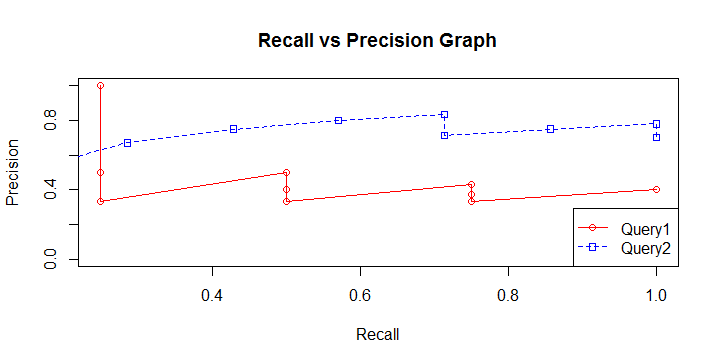
\includegraphics[width=1\textwidth]{Problem8_4/RecallvsPrecision.png}
  \caption{Recall vs Precision Graph}
  \label{fig:1}
\end{figure} 

\begin{figure}[ht]
  \centering
  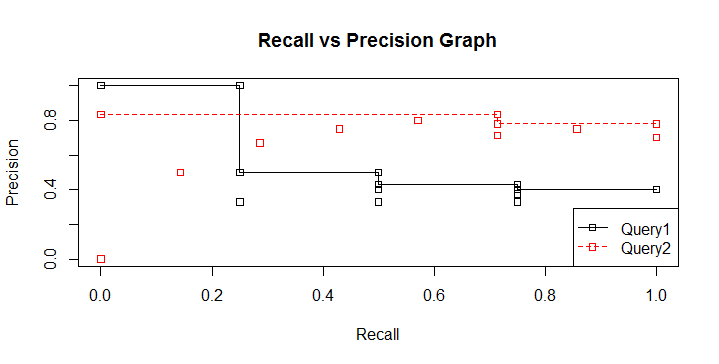
\includegraphics[width=1\textwidth]{Problem8_4/InterpolatedRecallvsPrecision.png}
  \caption{Interpolated Recall vs Precision Graph}
  \label{fig:1}
\end{figure}

\begin{table}[]
\centering
\caption{Precision values at standard recall levels calculated using interpolation}
\label{my-label}
\begin{tabular}{llllllllllll}
Recall          & 0.0   & 0.1   & 0.2   & 0.3   & 0.4   & 0.5   & 0.6   & 0.7   & 0.8  & 0.9  & 1    \\
Ranking 1       & 0.5     & 0.5     & 0.5     & 0.5   & 0.5   & 0.5   & 0.5 & 0.5 & 0.5  & 0.5  & 0.5  \\
Ranking 2       & 0.5     & 0.5     & 0.5     & 0.5   & 0.5   & 0.5   & 0.5 & 0.5 & 0.5  & 0.5  & 0.5  \\
Average Ranking  & 0.5     & 0.5     & 0.5     & 0.5   & 0.5   & 0.5   & 0.5 & 0.5 & 0.5  & 0.5  & 0.5  \\
\end{tabular}
\end{table}

\begin{figure}[ht]
  \centering
  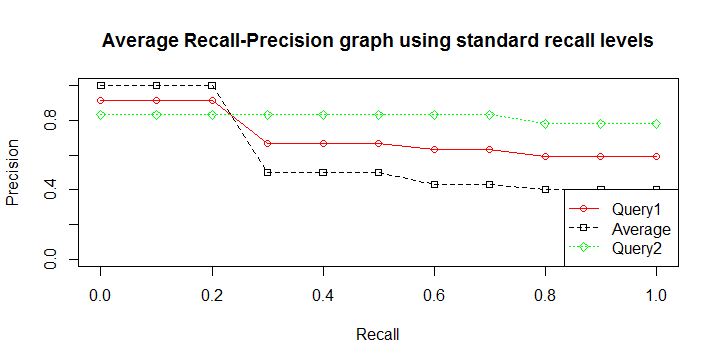
\includegraphics[width=1\textwidth]{Problem8_4/Averagerecallprecision.png}
  \caption{Average recall-precision graph using standard recall levels}
  \label{fig:1}
\end{figure}

Both the queries show their highest precision of 0.5 at recall value of 1. This results in a interpolated recall-precision graph to be a straight horizontal line at precision 0.5. Interpolated recall-precision graph is drawn with curves that are descending in manner, starting from highest point towards to lowest. But, for both the queries highest precision was reached at recall 1leading to a straight line.

\chapter{Problem 8.5}
\section{Problem}
Generate the mean average precision, recall-precision graph, average NDCG at 5 and 10, and precision at 10 for the entire CACM query set.
\section{Solution}
The results have been calculated by galago batch-search for rank result of 10. Galago provides NDCG 5 and 15 but not NDCG10. So, by making a request for 10 results per query the NDCG15 is same as NDCG10 beacause all the calculations are based on 10 results for each query.

The values for MAP is lesser than Precision at 10 for the CACM query set. Th query sets having most of their relevant results at top indexes (between 1 and 5) have higher or equal NCDG5 and NCDG10, but for queries with most of their relevant documents lower in the rank (between 6 and 10 ) have higher NCDG10 than NCDG5. 
\begin{figure}[ht]
  \centering
  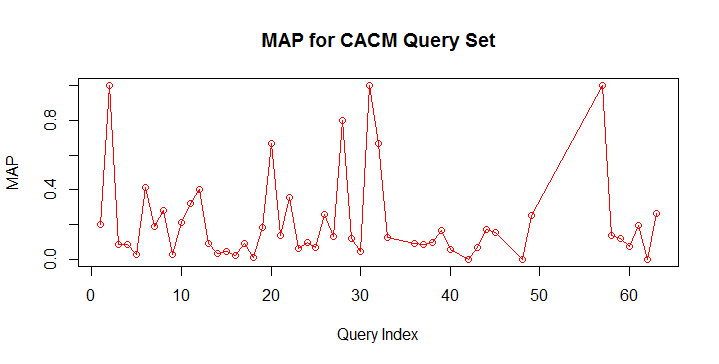
\includegraphics[width=1\textwidth]{Problem8_5/MAP.png}
  \caption{MAP values for CACM Query Set}
  \label{fig:1}
\end{figure}

\begin{figure}[ht]
  \centering
  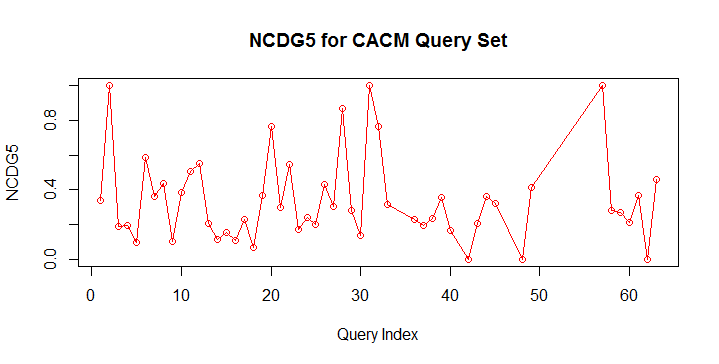
\includegraphics[width=1\textwidth]{Problem8_5/NCDG5.png}
  \caption{NCDG5 values for CACM Query Set}
  \label{fig:1}
\end{figure}

\begin{figure}[ht]
  \centering
  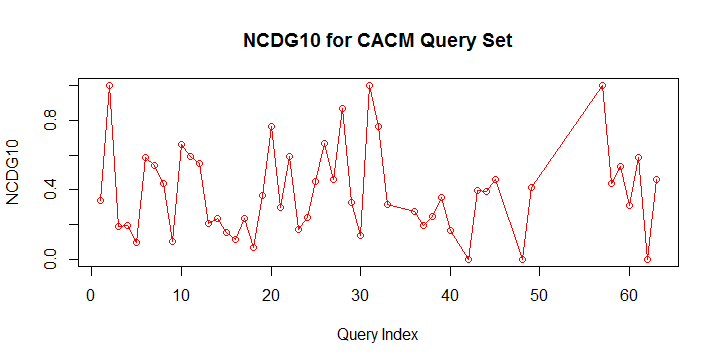
\includegraphics[width=1\textwidth]{Problem8_5/NCDG10.png}
  \caption{NCDG10 values for CACM Query Set}
  \label{fig:1}
\end{figure}

\begin{figure}[ht]
  \centering
  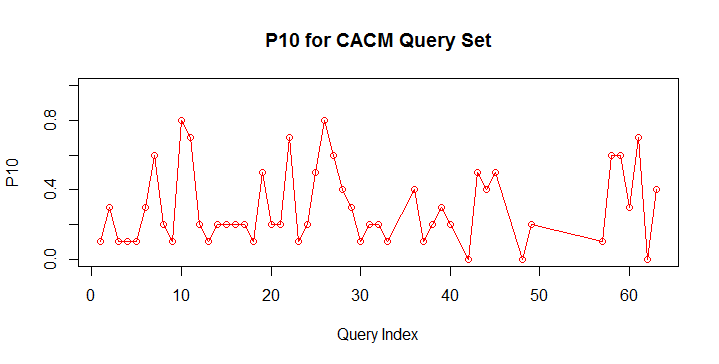
\includegraphics[width=1\textwidth]{Problem8_5/P10.png}
  \caption{Precision at 10 values for CACM Query Set}
  \label{fig:1}
\end{figure}

\begin{figure}[ht]
  \centering
  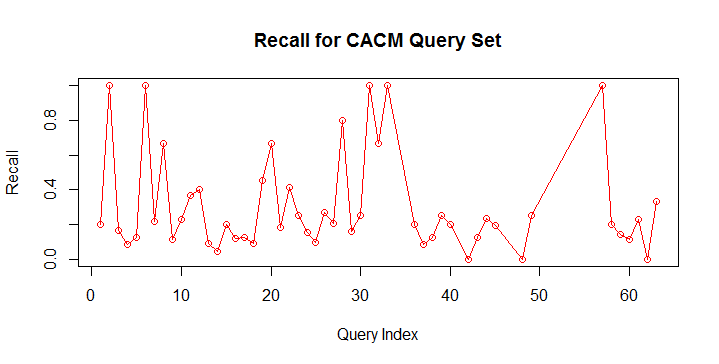
\includegraphics[width=1\textwidth]{Problem8_5/Recall.png}
  \caption{Recall values for CACM Query Set}
  \label{fig:1}
\end{figure}

\begin{figure}[ht]
  \centering
  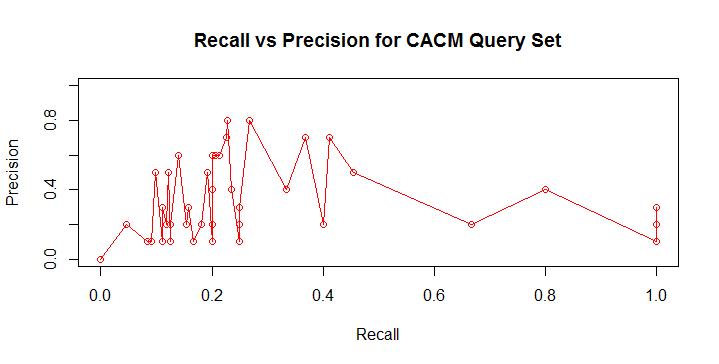
\includegraphics[width=1\textwidth]{Problem8_5/RecallvsPrecision.png}
  \caption{Recall vs Precision for CACM Query Set}
  \label{fig:1}
\end{figure}

\chapter{Problem 8.7}
\section{Problem}
Another measure that has been used in a number of evaluations is R-precision. This is defined as the precision at R documents, where R is the number of relevant documents for a query. It is used in situations where there is a large variation in the number of relevant documents per query. Calculate the average R-precision for the CACM query set and compare it to the other measures.
\section{Solution}
R-precision is defined as precision at R documents, where R is the number of relevant documents for a query. In context to the CACM query set, the relevance judgements file suggests that all the queries have varied number of relevant documents. It ranges from 0 to 51. So, for calculating R-precision number of relevant documents per query is set to 51 and evaluated in the galago.
The results for the different measures inclusive of R-precision at relevant document 51 are ahown in the table:


\begin{table}[]
\centering
\caption{CACM Query Set measured against different measures}
\label{my-label}
\begin{tabular}{llllllllllll}
map          &0.2840  \\
ndcg         &  0.4419     \\
ndcg15     & 0.4734  \\
R-prec      & 0.3192 \\
bpref        & 0.0000 \\
recip\_rank & 0.7296 \\
P5            & 0.3922 \\
P10          & 0.2980 \\
P15          & 0.2614 \\
P20          & 0.2373 \\
P30          & 0.1843  
\end{tabular}
\end{table}

\chapter{Problem 8.9}
\section{Problem}
For one query in the CACM collection, generate a ranking and calculate BPREF. Show that the two formulations of BPREF give the same value.
\section{Solution}
The solution is based on relevance results for query, interested in articles on robotics  motion planning particularly the geometric and combinatorial aspects   we are not interested in the dynamics of arm motion . The Table 5.1 shows the relevance results for the query. The relevance results show the search results had 3 relevant documents and 7 non- relevant documents. 

\verbatiminput{Problem8_3/cacm_onequery.list}

\subsection{Calculating BPREF}

$BPREF = 1/R \sum\limits_{d_r}^{}(1- ({N_{d_r}} / min(R,N))$

where R is the number of relevant documents that are considered\\
N is the number of non-relevant documents that are considered\\
$d_r$ is the number of relevant documents\\
 
For a query result with 3 relevant documents R is 3 implying that first 3 non-relevant documents are considered. The relevance table for the query is manipulated for BPREF as,\\

\begin{table}[]
\centering
\caption{Relevance table showing R relevant and non-relevant documents}
\label{my-label}
\begin{tabular}{ll}
Index & Relevance \\
1     & No       \\
2     & No        \\
3     & Yes        \\
4     & No       \\
5     & Yes        \\
6     & Yes      

\end{tabular}
\end{table}
$BPREF = 1/R \sum\limits_{d_r}^{}(1- ({N_{d_r}} / min(R,N))$\\
$BPREF = 1/3[(1-2/3) + (1 - 3/3) + (1- 3/3)]$\\
$BPREF = 1/3 [(1/3) + 0 + 0] = 3/8 = 0.11$

\subsection{Calculating BPREF based on preference}

$BPREF = P /( P + Q)$\\
where P is the number of relevant documents \\
          Q is the number of non-relevant documents\\
For query: Code optimization for space efficiency\\
P = 3\\
Q = 3\\
$BPREF = 3/(3+3)$\\
$BPREF = 0.5$\\

The value of BPREF is 0.11 and 0.3 by computing respectively with relevant documents formula and the clickthrough preference formula. The values computed are not equal because the bpref for clickthough formula does not take into account the ranking of relevant results and the value for BPREF with relevant documents formula dips due to the fist relevant result showing aftr two non-relevant result and the rest two relevant result appear after all the non-relevant documents taken in consideration. Thus, the last wo relevant documents do not add any value to the BPREF.
 
\chapter{Problem 9.8}
\section{Problem}
Cluster the following set of two-dimensional instances into three clusters using each of the five agglomerative clustering methods:
(–4, –2), (–3, –2), (–2, –2), (–1, –2), (1, –1), (1, 1), (2, 3), (3, 2), (3, 4), (4, 3)
Discuss the differences in the clusters across methods. Which methods produce the same clusters? How do these clusters compare to how you would manually cluster the points?
\section{Solution}
The code for agglomerate clustering methods generates 3 clusters for the data set.
\subsection{Discussion of the Methods}
Single Linkage: It uses the minimum distance between between elements of two clusters to merge them as one cluster. For two clusters A and B, it finds the minimum euclidean distance between the points of each cluster and compares them against the minimum threshold distance of all the other clusters to merge them in one cluster. The disadvantage of this approach is that it does not consider how far spread each cluster is and focusing only on the minimum distance between the clusters to merge them.\\ \\
Complete Linkage: It uses the maximum distance between elements of two clusters to merge them as one cluster. For two clusters A and B, it finds the maximum euclidean distance between the points of each cluster and compares them against the minimum distance of all the other clusters to merge them in one cluster. This approach creates a more comapact and less spread cluster than single linkage clustering technique.\\ \\
Average Clustering: It uses average distance of all the elements between two clusters to merge them as one cluster. For two clusters A and B, it finds the average distance by calculating the euclidean distance between all the points in each cluster and dividing them by the number of elements  in each cluster. The average distance calculated is compared against average distance of other clusters to merge the minimum average distance clusters in to one cluster. The type of cluster formed by average linkage depend heavily on the structure of clusters, since it is based on the average distance between all the elements in the two clusters. \\ \\
Average Group Clustering: It uses centroid distance between teo clusters to merge them as one cluster. For two clusters A and B, it finds the centroid of the two clusters and merges them together by comparing against the centroid distances of other clusters. It forms similar clusters to the average linkage clusters.\\ \\
Ward's Method: It uses sum of variance between two clusters to merge them as one cluster.It forms minimum spread clusters around the centroid of the cluster.\\
\lstinputlisting[language=Python]{Problem9_8/Clustering.py}
\verbatiminput{Problem9_8/ClusteringOutput.txt}
\subsection{Clustering Results vs Mannual Clustering }
All the agglomerate clustering techniques except for complete linkage technique produced the same result for the provided dataset. The results of the clusters formed by all the clustering methods has been shown above.\\
Mannual Clustering of the data points on euclidean distance results in the same clusters generated by agglomerative clustering.\\
Cluster 1: (-4,-2), (-3,-2), (--2,-2), (-1,-2)\\
Cluster 2: (1,-1), (1,1)\\
Cluster 3: (2,3), (3,2), (3,4), (4,3)\\
Cluster 1 is easy to create due to it being far away from other data points. Cluster 2 and 3 have a close margin where the distance between point (1,1) and (-1,1) is equal to 2 and the distance between point (1,1) and (2,3) is $\sqrt{5}$. Therefore the points (1,1) and (-1,1) have been clustered together as Cluster 2.\\
If the data points are clustered on the basis of the quadrants they lie in:\\
Cluster 1: 1st Quadrant$ ->$ (-4,-2), (-3,-2), (--2,-2), (-1,-2)\\
Cluster 2: 3rd Quadrant$ ->$ (1,-1)\\
Cluster 3:  4th Quadrant$ ->$ (1,1), (2,3), (3,2), (3,4), (4,3)\\
\chapter{9.9}
\section{Problem}
Use K-means and spherical K-means to cluster the data points in Exercise 9.8. How do the clusterings differ?
\section{Solution}
\lstinputlisting[language=Python]{Problem9_9/KMeans.py}
\verbatiminput{Problem9_9/Kmeans.txt}
The output of the code shows clusters on the basis of the index of data points and center of each cluster.Table 5.1 shows the index to data point relationship.The results for cluster size 2,3 and 4 are show for both the clustering techniques.\\
\begin{table}[]
\centering
\caption{Index  to Data Point relation}
\label{my-label}
\begin{tabular}{lllllllllll}
Index      & 0        & 1       & 2       & 3       & 4      & 5     & 6     & 7     & 8     & 9     \\
Data Point & (-4, -2) & (-3,-2) & (-2,-2) & (-1,-2) & (1,-1) & (1,1) & (2,3) & (3,2) & (3,4) & (4,3)
\end{tabular}
\end{table}
The clusters formed by K-means for cluster size 3 are same as the clusters formed by Single Linkage, Average Linkage and Average Group Linkage from the problem 9.8. The clusters formed by spherical K-means for cluster 3 is different from K-means due to the difference between finding similarity between points for clustering. K-means uses euclidean distance to find similarity while spherical K-mean uses cosine similarity to cluster items together. Spherical K-means clusters items on which fall in the ame quadrant approach discussed in the previous problem.\\
\chapter{Problem 9.11}
\section{Problem}
The K nearest neighbors of a document could be represented by links to those documents. Describe two ways this representation could be used in a search application.
\section{Solution}
The primary advantage of K nearest neighbor comapared to K means and agglomerative clustering techniques is that a document can be present in multiple clusters unlike the K means and agglomerative clustering technique where each documents is in a single cluster.\\

The K nearest neighbors of a documents can be used for tell-text search in search application. All the documents in the corpus can be clustered by K nearest neighbour. The document can be in multiple clusters based on the features extracted from the cluster. For a corpus of documents containing sports news from USA, it can be classified into multiple clusters as football, baseball, basketball, athletics, Olympics, CONCAF Cup etc. A document that is in cluster soccer can simultaneously be clustered with Olympics and CONCAF Cup. Similarly the queries to the documents can also be clustered on the basis of its features. It presents all the documents that are in the cluster soccer for a query of feature soccer. The same set of documents can also be recalled if the query is about CONCAF Cup. It allows for relavant search results.\\

The K nearest neighbors can also be used for showing clustered search results. It can be helped to refine a very generic query to a more precise query to return relevant result. For example, a system that employs K nearest neighbor clustering on its queries. For a user input query apple, it will show all the possible clusters where the query term apple appears. For apple, it can be a fruit, it can be the company Apple, it can be products of Apple Company etc. A user on the basis of suggestions can select the particular suggestion  to find search results that fall under the specified feature cluster.\\ 
  
   
   




  


\end{document}